% !TeX root = ../Book3.tex
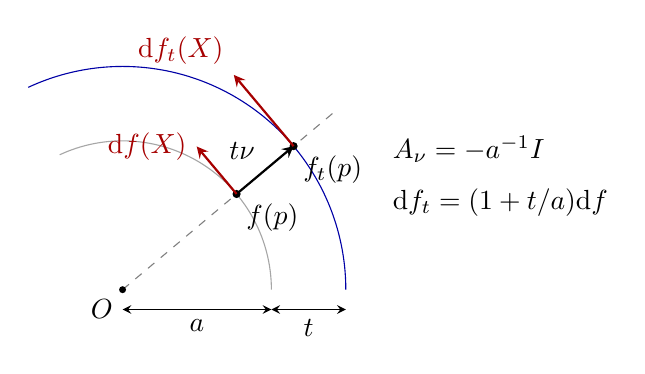
\begin{tikzpicture}[scale=1.05,>=stealth]
	\draw[gray!70] (0:1.8) arc[start angle=0,end angle=115,radius=1.8];
	\draw[blue!65!black] (0:2.7) arc[start angle=0,end angle=115,radius=2.7];
	\draw[gray,dashed] (0,0)--(40:3.35);
	\coordinate (P) at (40:1.8);
	\coordinate (Q) at (40:2.7);
	\fill (0,0) circle (1.2pt) node[below left]{\(O\)};
	\fill (P) circle (1.4pt) node[below right]{\(f(p)\)};
	\fill (Q) circle (1.4pt) node[below right]{\(f_t(p)\)};
	\draw[->,thick] (P)--(Q) node[midway,above left]{\(t\nu\)};
	\draw[->,thick,red!65!black] (P)--++(130:0.75) node[left]{\(\mathrm df(X)\)};
	\draw[->,thick,red!65!black] (Q)--++(130:1.125) node[above left]{\(\mathrm df_t(X)\)};
	\draw[<->] (0,-0.24)--(1.8,-0.24) node[midway,below]{\(a\)};
	\draw[<->] (1.8,-0.24)--(2.7,-0.24) node[midway,below]{\(t\)};
	\node[anchor=west] at (3.15,1.7){\(A_\nu=-a^{-1}I\)};
	\node[anchor=west] at (3.15,1.05){\(\mathrm df_t=(1+t/a)\mathrm df\)};
\end{tikzpicture}
